\chapter{Primer on UAVs}

\section{History of Drones}
\label{sec:drone-history}

Unmanned aerial vehicles (UAVs), or drones, are aircraft that can be operated
remotely without the need for a human pilot on board. While there were many
early pilotless aircraft, the first remote controlled aircraft appeared during
the First World War, developed by Britain and the US in 1917
\cite{dronehistory}. Many of these early drones were used as anti-aircraft
gunnery training targets. In the 1930s, the term "drone" arose inspired by the
de Havilland DH82B Queen Bee (\cref{fig:queen-bee}), designed as a low-cost
radio-controlled target aircraft, which saw over four hundred units built by
1943. The Queen Bee was the first drone designed with the ability to return to
ground safely and be reused \cite{queenbee, pbs05}.

\begin{figure}[htbp]
\centerline{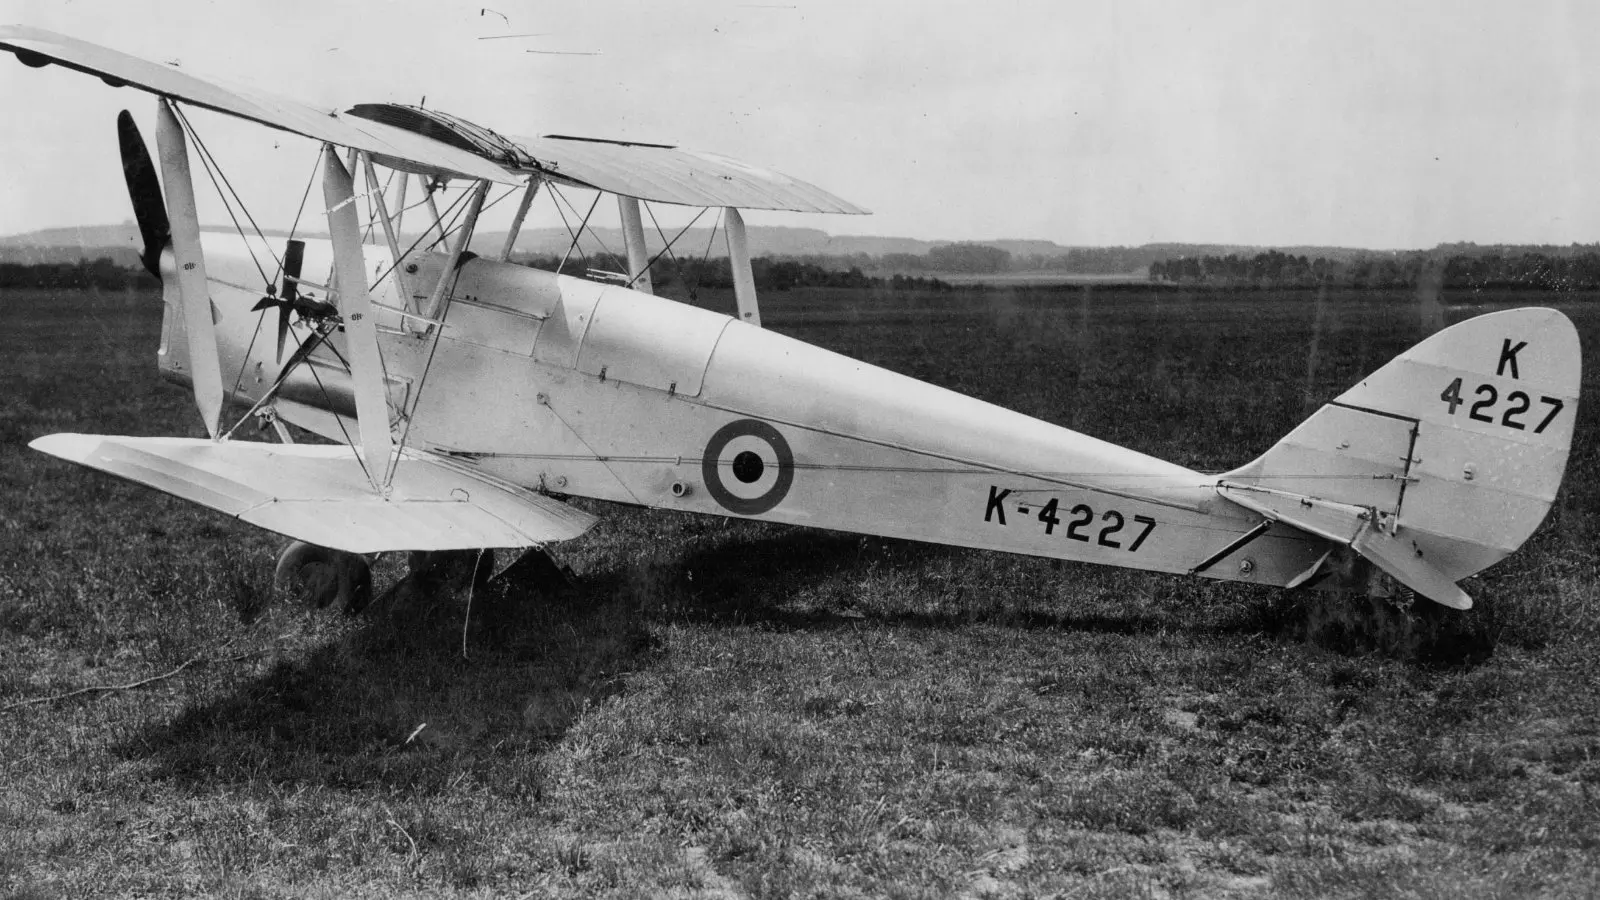
\includegraphics[width = .6\textwidth]{figs/queenbee.png}}
\caption{de Havilland DH82B Queen Bee \cite{baesystems}, the first radio-controlled drone}
\label{fig:queen-bee}
\end{figure}

These early drones were fixed-wing aircraft that were used primarily for combat
or training. From the 1970s, drones such as the Ryan Model 147 Lightning
Bugdrones were developed for use in surveillance missions. These drones carried
a camera and could fly for hours at high altitude \cite{pbs12}. The Pioneer
UAV, introduced in 1986, saw extensive use in the Gulf War. Today, the General
Atomics MQ-1 Predator can fly for over 14 hours performing surveillance
missions using an array of sensors, including infrared cameras.

The turn of the century saw the use of small drones in civillian settings, with
technology advances making them cheaper to produce. Drones, particularly
quadcopters (\cref{fig:dji-mini-4k}), started being used for mapping, aerial
photography, industrial inspections and security, and precision agriculture
\cite{giones2017}. Compared to previous fixed-wing military drones, quadcopters
offer superior maneuverability and the ability to hover. They utilize four
motor-rotors, with two spinning clockwise and the other two counterclockwise.
Variations in motor speed allow for precise hovering and maneuverability. This
makes quadcopter drones well-suited for both indoor and outdoor use.  Since the
2010s, drones have evolved significantly, with a range of consumer photography
and racing drones easily available to consumers, at a wide range of price
points. Drones are commonly used for filming and recreation, and have also seen
use in logistics, to deliver packages. The scale of their adoption is
immense---The Federal Aviation Administration (FAA) has received registrations
for almost 800,000 drones \cite{faa_drones_2024}.  This figure excludes
thousands of hobbyist drones weighing under 250 g that do not require FAA
registration.

\section{The capabilities of today's drones}
\label{sec:drone-capabilities}

\begin{figure}[htbp]
\centerline{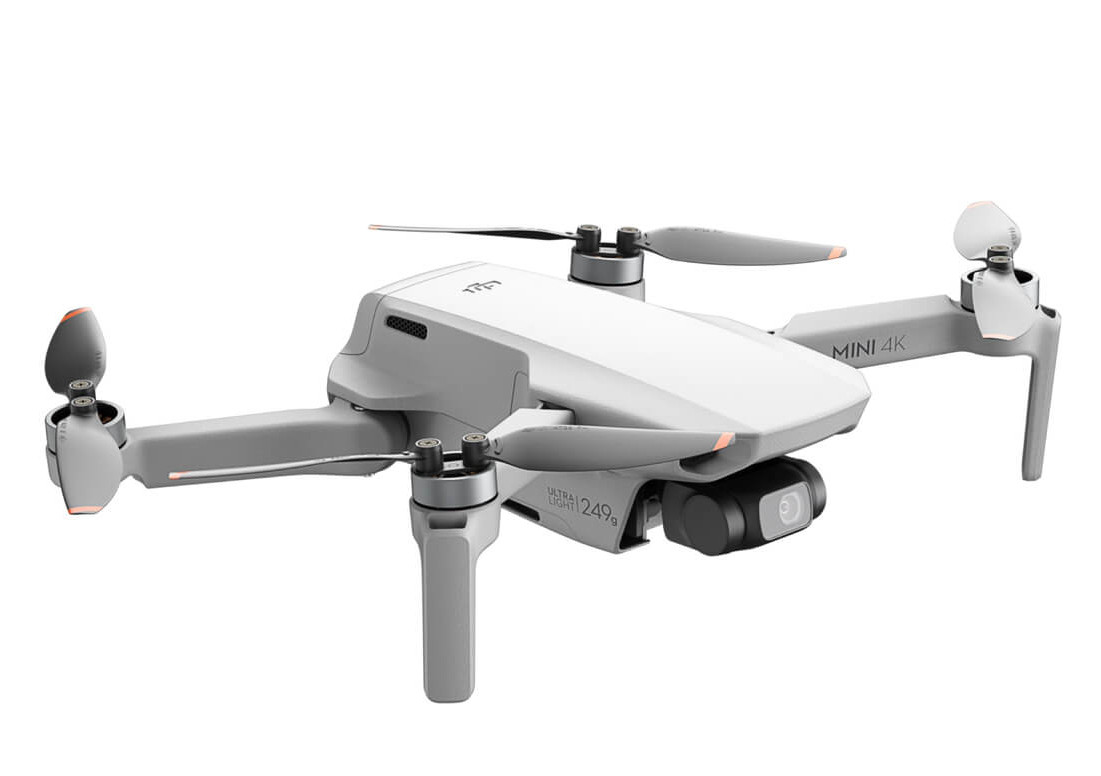
\includegraphics[width = .5\textwidth]{figs/dji-mini-4k.jpg}}
\caption{DJI Mini 4K}
\label{fig:dji-mini-4k}
\end{figure}

Today, the set of features available in consumer-grade drones is impressive.
The DJI Mini 4K, for instance, is priced at \$299, weighs under 250g, records
video at 4K 30 FPS, and has a maximum flight time of about 30 minutes
\cite{dji_mini_4k}. Most drone's today have the ability to fly
semi-autonomously in addition to the ability to be controlled remotely by a
human. As shown in \cref{fig:drone-components}, drones have advanced
microprocessors that abstract away the lower-level mechanics of quadcopter
drone flight. Components such as the Electronic Speed Controller (ESC) enable
precise control of the drone's brushless electric motors. On-board positioning
systems such as Global Navigation Satellite System (GNSS) receivers give the
drone the ability to navigate between waypoints.  Using inputs from on-board
intertial measurement unit (IMU) sensors such as gyroscopes, accelerometers,
and magnetometers, drones can determine their orientation, acceleration, and
rotation, allowing them to adjust their motors in real-time to counter wind and
hover in a fixed position. They can also typically takeoff and land
autonomously. On-board flight control software such as PX4 or ArduPilot, also
known as an "autopilot," makes these higher-level functions possible, taking
inputs from the IMU and GNSS sensors and outputting control commands to the
ESC.

\begin{figure}[htbp]
\centerline{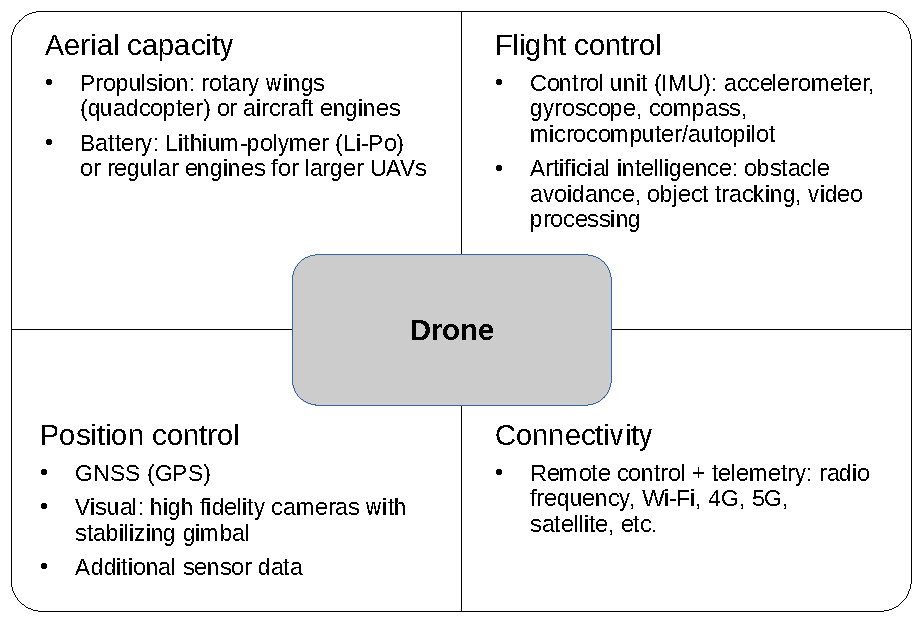
\includegraphics[width = .6\textwidth]{figs/drone-components-crop.pdf}}
\caption{Components of a drone \cite{giones2017}}
\label{fig:drone-components}
\end{figure}

Drones are equipped with a variety of cameras, such as monocular and stereo.
Monocular cameras capture images and videos from a single point of view, and
are common in consumer aerial photography drones. Monocular cameras are often
mounted on a gimbal, which stabilizes the drone's camera during motion and also
allows the ability to capture different viewing angles through gimbal motion.
Stereoscopic cameras, on the other hand, offer multiple point of views. Having
more than one camera allows the use of epipolar geometry and triangulation to
determine distance from objects efficiently, and perform obstacle avoidance.
The DJI Mini 4 Pro, for instance, has multiple binocular cameras, facing
forward, backward, sideways, upwards, and downwards. This allows the Mini 4 Pro
to perform omnidirectional obstacle sensing. During manual pilot flight, the
drone offers pilot assistance features that stop the drone if it is headed for
an imminent collision, and also provide the option to circumvent obstacles
automatically altogether. Drones equipped with monocular cameras typically lack
these advanced obstacle avoidance systems, but are cheaper and more common.

While consumer-grade drones offer many semi-autonomous features, complex
fully-autonomous features are limited to more expensive commerical drones.  For
example, a consumer drone could be instructed to navigate to a given GPS
coordinate or, in some advanced drones, even track an on-ground target. But
complex missions, such as patrolling a set of waypoints while searching for an
on-ground target, and transitioning to track the target once it is detected,
remain out of the reach of consumer drones.

Consumer drones are typically controlled over Wi-Fi using a controller or a
smartphone app, and typically lack cellular connectivity, limiting their
flying range.


